\section{Exercise 04}
\subsection{}

\begin{frame}[label={pag:ex-realisation}]
\frametitleTC{Problem}
\framesubtitleTC{This one we solve together}
\myPause
 Take the block diagram
 \begin{center}
  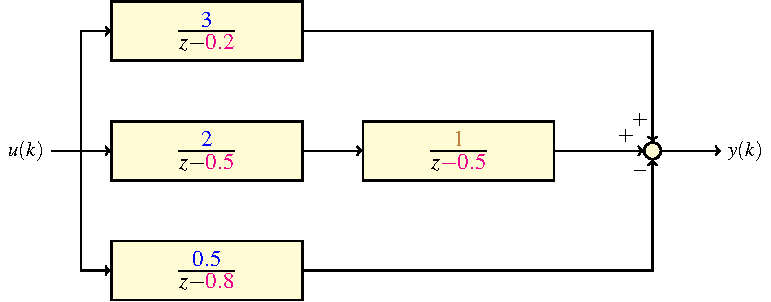
\includegraphics[width=0.85\columnwidth]{./Unit-03/img/PS01-ex04-fig01.pdf}
 \end{center}\myPause
 \begin{itemize}[<+-| alert@+>]
 \item[(a)] compute the transfer function from $u(k)$ to $y(k)$,
 \item[(b)] find a possible state-space description for the system.
 \end{itemize}
\end{frame}

\begin{frame}
\frametitleTC{Solution}
\framesubtitleTC{Item (a) -- preliminaries}
\myPause
 \begin{itemize}[<+-| alert@+>]
 \item Take two blocks in \TC{series} or \TC{cascade}, i.e., the output $y_1(k)$ of the first is the
       input $u_2(k)$ of the second. Name $G_1(z)$ and $G_2(z)$ their transfer functions.
 \item Let the overall system input $u(k)$ be connected to the input $u_1(k)$ of $G_1(z)$, and the overall
       system output $y(k)$ be the output $y_2(k)$ of $G_2(z)$.
 \item Then we have
       \begin{displaymath}
        y(k) = y_2(k) = G_2(z)u_2(k) = G_2(z)y_1(k) = G_2(z)G_1(z)u_1(k)=G_2(z)G_1(z)u(k),
       \end{displaymath}
 \item and therefore the overall transfer function $G(z)$ from $u(k)$ to $y(k)$ is
       \begin{displaymath}
        G(z) = G_2(z)G_1(z).
       \end{displaymath}
 \end{itemize}
\end{frame}

\begin{frame}
\frametitleTC{Solution}
\framesubtitleTC{Item (a) -- preliminaries}
\myPause
 \begin{itemize}[<+-| alert@+>]
 \item Take two blocks $G_1(z)$ and $G_2(z)$ in \TC{parallel}, i.e., they get the same input $u(k)$
       and their outputs sum together to produce the overall system output $y(k)$.
 \item With obvious notation have
       \begin{displaymath}
        y(k) = y_1(k)+y_2(k) = G_1(z)u_1(k)+G_2(z)u_2(k) = (G_1(z)+G_2(z))u(k),
       \end{displaymath}
 \item and therefore the overall transfer function $G(z)$ from $u(k)$ to $y(k)$ is
       \begin{displaymath}
        G(z) = G_1(z)+G_2(z).
       \end{displaymath}
 \item Extending to more blocks and different signs is trivial.
 \end{itemize}
\end{frame}

\begin{frame}
\frametitleTC{Solution}
\framesubtitleTC{Item (a)}
\myPause
 \begin{itemize}[<+-| alert@+>]
 \item The system under question is composed of three branches in parallel.
 \item The middle one is composed of two blocks in series.
 \item Hence (mind the signs) the overall transfer function $G(z)=y(k)/u(k)$ is
       \begin{displaymath}
        \begin{array}{rcll}
         G(z) &=& & \cfrac{3}{z-0.2}\\
              & &+& \cfrac{2}{z-0.5} \,\cdot\,
                    \cfrac{1}{z-0.5}\\
              & &-& \cfrac{0.5}{z-0.8} \; \ldots\\ \\
              &=& & \cfrac{2.5z^3-2.8z^2+0.925z-0.255}{(z-0.2)(z-0.5)^2(z-0.8)}.
        \end{array}
       \end{displaymath}
 \end{itemize}
\end{frame}

\begin{frame}
\frametitleTC{Solution}
\framesubtitleTC{Item (b)}
\myPause%
 \only<2 >{Consider the individual first-order blocks:\\%
           \begin{center}
            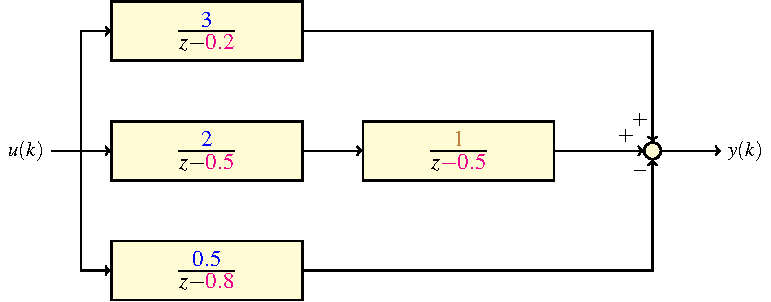
\includegraphics[width=0.85\columnwidth]{./Unit-03/img/PS01-ex04-fig01.pdf}
           \end{center}}
 \only<3 >{Take their outputs as state variables:\\%
           \begin{center}
            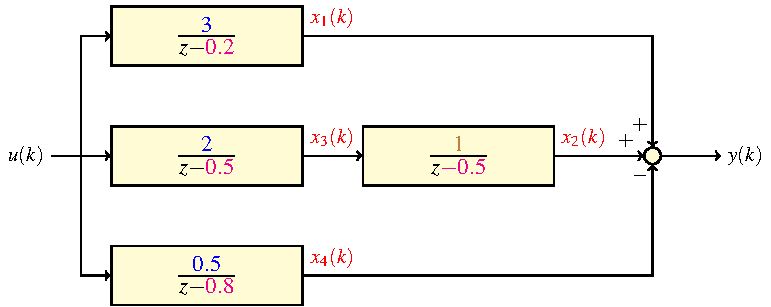
\includegraphics[width=0.85\columnwidth]{./Unit-03/img/PS01-ex04-fig02.pdf}
           \end{center}}
 \only<4->{write the elementary difference equations for each block:\\%
           \begin{center}
            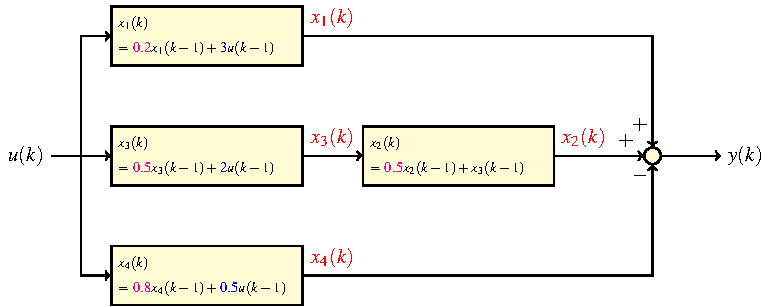
\includegraphics[width=0.85\columnwidth]{./Unit-03/img/PS01-ex04-fig03.pdf}
           \end{center}}
\end{frame}

\begin{frame}
\frametitleTC{Solution}
\framesubtitleTC{Item (b)}
\myPause
 \begin{itemize}[<+-| alert@+>]
 \item Now put it all together:
       \begin{displaymath}
        \left\{\begin{array}{rlllll}
         x_1(k) &= 0.2x_1(k-1) &              &              &              & +u(k-1)    \\
         x_2(k) &=             & +0.5x_2(k-1) & +x_3(k-1)                                \\
         x_3(k) &=             &              &  0.5x_3(k-1) &              & +2u(k-1)   \\
         x_4(k) &=             &              &              &  0.8x_4(k-1) & +0.5u(k-1) \\
         y(k)   &= x_1(k)      & +x_2(k)      &              & -x_4(k)                   \\
        \end{array}\right.
       \end{displaymath}
 \item Hence
       \begin{displaymath}
        \begin{array}{c}
         A = \begin{bmatrix}
              0.2 & 0   & 0   & 0   \\
              0   & 0.5 & 1   & 0   \\
              0   & 0   & 0.5 & 0   \\
              0   & 0   & 0   & 0.8
             \end{bmatrix}, \quad
         b = \begin{bmatrix} 1 \\ 0 \\ 2 \\ 0.5 \end{bmatrix}, \\ \\
         c = \begin{bmatrix} 1 & 0 & 1 & -1 \end{bmatrix}, \quad
         d = 0.
        \end{array}
       \end{displaymath}
 \end{itemize}
\end{frame}

\begin{frame}
\frametitleTC{Takeaways}
\framesubtitleTC{from exercise 04}
\myPause
 \begin{itemize}[<+-| alert@+>]
 \item We know that the poles of $G(z)$ are eigenvalues of $A$.
 \item Not THE eigenvalues, some may be cancelled.
 \item Our matrices are real, hence eigenvalues (and poles) are either real, or in complex
       conjugate couples. Here we limit the math to real ones (but results hold in general).
 \item \vfill It should be clear that \emph{any} $G(z)$, once decomposed in simple fractions,\\
       can be treated as we did.
 \item Can we say something on our $A$? Can we use it to understand\\
       the eigenvalues--stability relationship we mentioned? 
 \item Remember that the free motion of a system converges to zero,\\
       diverges or neither, if so  does $A^k$ for $k\rightarrow\infty$. Let us have a look\\
       with this idea in mind.
 \end{itemize}
\end{frame}

\begin{frame}
\frametitleTC{Takeaways}
\framesubtitleTC{from exercise 04}
\myPause
 \begin{itemize}[<+-| alert@+>]
 \item In general, once treated as we did, matrix $A$ looks e.g. as follows:
 \begin{displaymath}
  A = 
  \begin{bmatrix}
   \-& \cellcolor{green!30!white}{\lambda_{1}} & 0 & 0 & 0 & 0 & 0 & 0 & \ldots & \\
   \-& 0 &\cellcolor{green!30!white}{\lambda_{2}}  & 0 & 0 & 0 & 0 & 0 \\
   \-& 0 & 0 &\cellcolor{orange!50!white}{\lambda_{3}}
             &\cellcolor{yellow!30!white}{\textcolor{cyan!80!black}{0}} & 0 & 0 & 0 \\
   \-& 0 & 0 &\cellcolor{yellow!30!white}{0}
             &\cellcolor{orange!50!white}{\lambda_{3}} & 0 & 0 & 0 \\
   \-& 0 & 0 & 0 & 0 &\cellcolor{orange!50!white}{\lambda_{4}}
                     &\cellcolor{orange!30!white}{\textcolor{red}{1}} & \cellcolor{yellow!30!white}{0} \\
   \-& 0 & 0 & 0 & 0 &\cellcolor{orange!30!white}{0}
                     &\cellcolor{orange!50!white}{\lambda_{4}}
                     & \cellcolor{yellow!30!white}{\textcolor{cyan!80!black}{0}} \\
   \-& 0 & 0 & 0 & 0 &\cellcolor{yellow!30!white}{0}
                     &\cellcolor{yellow!30!white}{0} & \cellcolor{orange!50!white}{\lambda_{4}} \\
   \-& \vdots &&&&&&& \ddots \\
  \end{bmatrix}
 \end{displaymath}
 \item Notice the block diagonal structure:
       \begin{itemize}[<+-| alert@+>]
       \item \colorbox{green!30!white}{single} eigenvalues are just diagonal elements;
       \item \colorbox{orange!50!white}{multiple} ones are repeated to form square \colorbox{yellow!30!white}{blocks},
       \item in turn diagonally composed of \colorbox{orange!30!white}{mini-blocks} separated by
             \textcolor{cyan!80!black}{zeroes}\\
             that break the over-diagonal sequence of \textcolor{red}{ones} in the block.
       \end{itemize}
 \end{itemize}
\end{frame}

\begin{frame}
\frametitleTC{Takeaways}
\framesubtitleTC{from exercise 04}
\myPause
 \begin{itemize}[<+-| alert@+>]
 \item Now, let us compute $A^k$:\myPause
 \begin{displaymath}
  A^k = 
  \begin{bmatrix}
   \-& \cellcolor{green!30!white}{\lambda_{1}^k} & 0 & 0 & 0 & 0 & 0 & 0 & \ldots & \\
   \-& 0 &\cellcolor{green!30!white}{\lambda_{2}^k}  & 0 & 0 & 0 & 0 & 0 \\
   \-& 0 & 0 &\cellcolor{orange!50!white}{\lambda_{3}^k}
             &\cellcolor{yellow!30!white}{\textcolor{cyan!80!black}{0}} & 0 & 0 & 0 \\
   \-& 0 & 0 &\cellcolor{yellow!30!white}{0}
             &\cellcolor{orange!50!white}{\lambda_{3}^k} & 0 & 0 & 0 \\
   \-& 0 & 0 & 0 & 0 &\cellcolor{orange!50!white}{\lambda_{4}^k}
                     &\cellcolor{orange!30!white}{\textcolor{red}{k\lambda_4^{k-1}}} & \cellcolor{yellow!30!white}{0} \\
   \-& 0 & 0 & 0 & 0 &\cellcolor{orange!30!white}{0}
                     &\cellcolor{orange!50!white}{\lambda_{4}^k}
                     & \cellcolor{yellow!30!white}{\textcolor{cyan!80!black}{0}} \\
   \-& 0 & 0 & 0 & 0 &\cellcolor{yellow!30!white}{0}
                     &\cellcolor{yellow!30!white}{0} & \cellcolor{orange!50!white}{\lambda_{4}^k} \\
   \-& \vdots &&&&&&& \ddots \\
  \end{bmatrix}
 \end{displaymath}\myPause
 \item Does it converge to a matrix of zeroes? Or diverge --- i.e., does\\
       at least one element diverge? Or neither?
 \item In other words, is the system asymptotically stable, unstable,\\
       or (simply) stable?
 \end{itemize}
\end{frame}

\begin{frame}[fragile]
\frametitleTC{Takeaways}
\framesubtitleTC{from exercise 04}
\myPause
 \begin{itemize}[<+-| alert@+>]
 \item Diagonal terms, in the form $\lambda^k$:
       \begin{displaymath}
        \begin{array}{rcl}
         \lim\limits_{k\rightarrow\infty}|\lambda^k| = 
          \begin{cases}
           0        & |\lambda| < 1 \\
           1        & |\lambda| = 1 \\
           \infty   & |\lambda| > 1 \\
          \end{cases}
        \end{array}
       \end{displaymath}
 \item Over-diagonal terms, in the form $k\lambda^k$:
       \begin{displaymath}
        \begin{array}{rcl}
         \lim\limits_{k\rightarrow\infty}|k\lambda^k| = 
          \begin{cases}
           0        & |\lambda| < 1 \\
           \infty   & |\lambda| \geq 1 \\
          \end{cases}
        \end{array}
       \end{displaymath}
 \item NOTE: larger mini-blocks give over-diagonal terms in other forms,\\
       but analogous as for the above. Take wxMaxima and try e.g.\\
       {\small
       \begin{verbatim}
  A:matrix([lambda,1,0],[0,lambda,1],[0,0,lambda]);
  A.A.A; /* NOT A^3, that is the elem-by-elem power */
       \end{verbatim}
       }
 \end{itemize}
\end{frame}

\begin{frame}
\frametitleTC{Takeaways}
\framesubtitleTC{from exercise 04}
\myPause
 \begin{itemize}[<+-| alert@+>]
 \item Now let us put it all together:
       \begin{itemize}[<+-| alert@+>]
       \item each single eigenvalue $\lambda_i$ only gives one diagonal term $\lambda_i^k$;
       \item each eigenvalue $\lambda_j$ with multiplicity $n_j$ gives $n_j$ diagonal terms $\lambda_j^k$, plus some\\
             \vspace{-0.75mm}over-diagonal terms $k\lambda_j^k$ -- or analogous -- iff the maximum size of its mini-block\\
             is greater then one.
       \end{itemize}
 \item Hence\\
       {\scriptsize 
       %\begin{center}
        \begin{tabular}{rcl}
         all $|\lambda_i|<1$                             & $\Rightarrow$ & System asymptotically stable\\
         \\
         at least one $|\lambda_i|>1$                    & $\Rightarrow$ & System unstable\\
         \\
         all $|\lambda_i|\leq 1$                         & \\
         and at least one has unity magnitude            & $\Rightarrow$ & System (simply) stable\\
         but in this case also unity max mini-block size & \\
         \\
         otherwise (i.e.,all $|\lambda_i|\leq 1$, and    & \\
         at least one has both unity magnitude and       & $\Rightarrow$ & System unstable\\
         maximum mini-block size greater than one)       & \\
        \end{tabular}
       %\end{center}
       }
 \item \vfill This proves (and completes) the statement of slide~\ref{pag:stab-eivals}.
 \end{itemize}
\end{frame}

 

